\section{Computer Arithmetic}
\begin{greenquote}
  In Spring 2025, this was the start of Lecture 1.
\end{greenquote}

We often want to work with the real number system, which consists of all 
integers, rational and irrational numbers
\begin{equation*}
  2, \sqrt{2}, e, \pi, 10^6, \text{ etc.} 
\end{equation*}
Because we have a finite space limitation for numbers, 
\textbf{not all numbers can be represented exactly.} This can cause problems
with arithmetic.

\subsection{Bases - Binary and Decimal}

We typically use the decimal (base 10) system, e.g.
\begin{equation*}
  427.325 = 4 \times 10^2 + 2 \times 10^1 + 7 \times 10^{0} + 3 \times 10^{-1}+\dots
\end{equation*}
However, when we work with a computer, we use the binary (base 2) system:
\begin{equation*}
  (1001.11101)_2 = 1\times 2^3 + 0\times 2^2 + 0\times 2 + 1\times 2^0 + 1\times 2^{-1} + 1\times 2^{-2} + 1\times 2^{-3} +\dots
\end{equation*}
In this class, we will only be working in the decimal system in order to make
computations simpler, since the application of concepts is identical.

\subsection{Base Conversion and Error}

Because it is impossible to represent some finite decimal fractions in binary,
we will (definitely) encounter \textbf{error} when converting from base-10 to
base-2. In the following example, we will convert $\frac{1}{10}$ to binary, and
show how there exists some numbers which cannot be represented exactly within 
the binary floating-point system.

% Notice that conversion from base-10 to base-2 can lead to errors. It is 
% impossible to represent some finite decimal fractions in binary.

\subsubsection{Example}

To convert a decimal fraction like $\frac{1}{10}$ into its binary 
representation, we repeatedly multiply the fractional part by $2$ and extract
the integer part at each step.

We begin with $1/10 = 0.1_{10}$, and assume $0.1_{10} = (a_1.a_2a_3\dots
a_n)_2$.
\[
\frac{1}{10} = 0.1_{10} = (0.a_1a_2a_3\dots a_n)_{2}
\]

Multiply by $2$:
\[
2 \times 0.1 = 0.2 = (a_1.a_2a_3\dots)_2
\]

Keep the fractional part and repeat:
\begin{align*}
  &a_1 = \lfloor 0.2 \rfloor = 0 \\
  2 \times 0.2 = 0.4 \implies &a_2 = \lfloor 0.4 \rfloor = 0 \\
  2 \times 0.4 = 0.8 \implies &a_3 = \lfloor 0.8 \rfloor = 0 \\
  2 \times 0.8 = 1.6 \implies &a_4 = \lfloor 1.6 \rfloor = 1 \\
  1.6 - 1 &= 0.6 \\
  2 \times 0.6 = 1.2 \implies &a_5 = \lfloor 1.2 \rfloor = 1 \\
  1.2 - 1 &= 0.2
\end{align*}

We have now returned to $0.2$, which was the value after the very first 
multiplication. This means the process will repeat indefinitely. Thus, the 
binary representation of $\frac{1}{10}$ is:
\[
  \frac{1}{10} = (0.0\mathbf{0011}00110011\dots)_2
\]
The repeating part is \textbf{0011}\dots, and this pattern continues forever. 
Using a finite number of digits, $\frac{1}{10}$ \textbf{cannot} be represented
exactly in binary. Just as $\frac{1}{3} = 0.\overline{3}$ cannot
be perfectly represented in decimal, the same is true for $\frac{1}{10}$ in
binary. This is why certain decimal fractions lead to rounding errors in binary-
based floating-point arithmetic.

\section{Hypothetical Storage Scheme (32-bit)}

We will use a hypothetical decimal computer since the concept is identical.
(By the way, this is very close to 
\ulhref{https://en.wikipedia.org/wiki/IEEE_754}{IEEE-754} floating point
representation, except that we are using a decimal representation instead of
binary.)

Suppose we have the decimal number $423.7$. Since we always want to represent
numbers in proper scientific notation, we normalize the
\textbf{mantissa}.
We write our number as follows:

\begin{equation*}
  423.7 = +\underbrace{0.4237}_{\text{mantissa}} \times 10^{+3}
\end{equation*}
Notice the $+$ is relevant because we require an explicit representation of the
sign of the number. We call the bits following from the decimal point ($4273$) 
the \textbf{mantissa}.
We include 1 bit for the sign, which is $1$ for positive numbers, 1 bit for the
exponent sign, 7 bits for the exponent, and the remaining 23 bits for the
mantissa.

\begin{figure}[h]
  \centering
  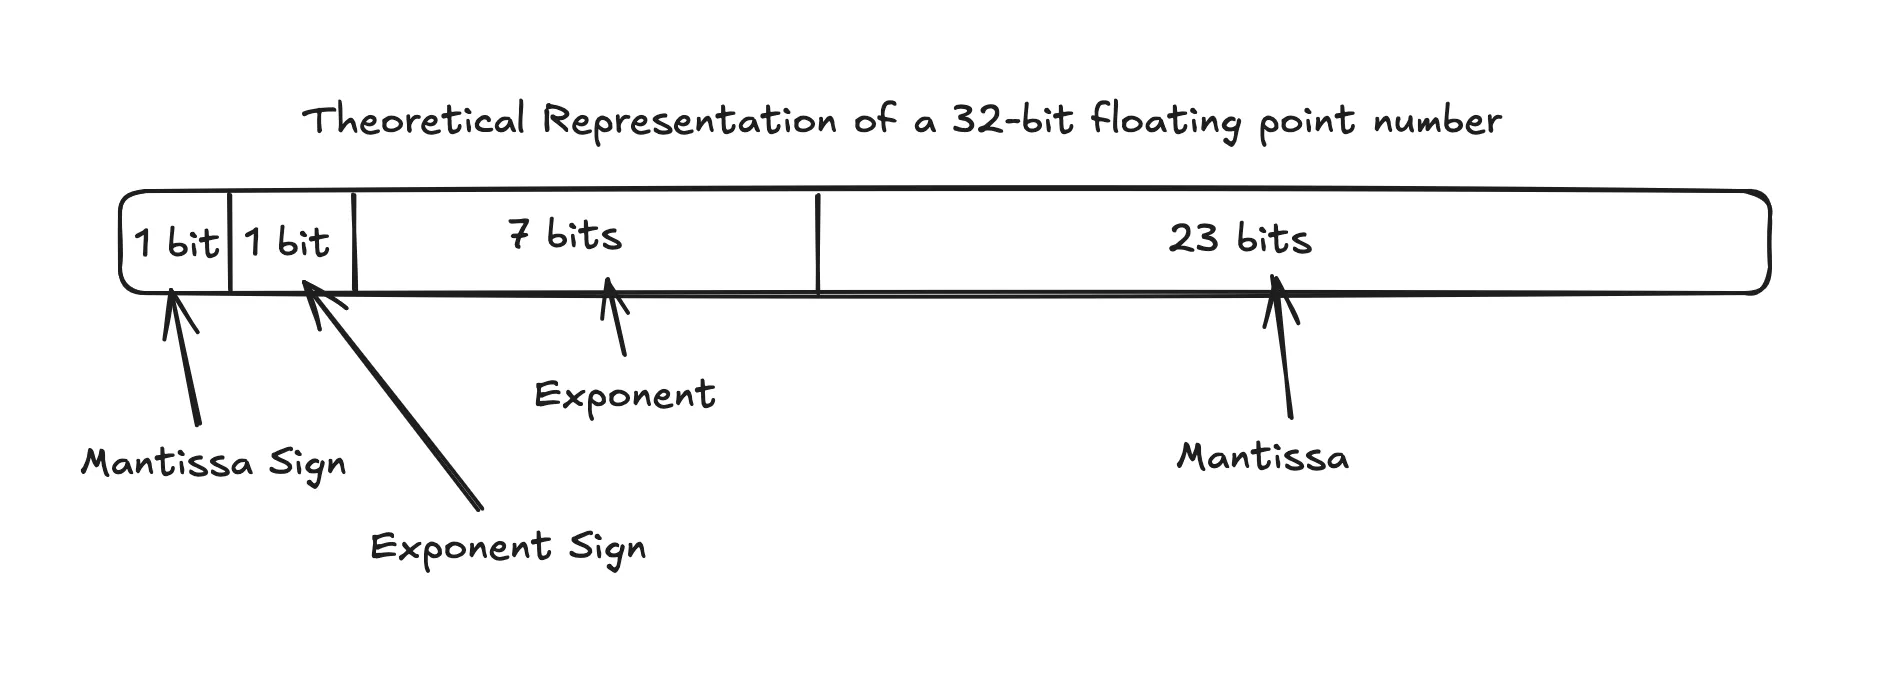
\includegraphics[width=0.8\textwidth]{./assets/fake_ieee754.png}
  \caption{Hypothetical Storage Scheme (32-bit)}
\end{figure}

\subsection{Problems with Floating Point}
\noindent
\begin{minipage}{\textwidth}
Because our storage format is finite, the biggest problems we will encounter
are:
\begin{enumerate}
  \item \textbf{bit overflow}: the maximum magnitude of our exponent (in binary)
    is \textbf{127}, so our number can only range from $2^{-127}$ to $2^{+127}$.
  \item \textbf{rounding error}: because our mantissa only has 23 bits of 
    precision, the precision will decrease as our numbers get larger because we 
    use exponentiation to represent the actual number.
\end{enumerate}
\end{minipage}

% Because our storage format is finite, one of the biggest problems we will 
% encounter is \textbf{bit overflow}. The maximum magnitude of our exponent 
% (in binary) is \textbf{127}, so our number can only range from $2^{-127}$ to
% $2^{+127}$. Because our mantissa only has 23 bits of precision, the precision
% will decrease as our numbers get larger because we use exponentiation to 
% represent the actual number.

\subsubsection{Error Example}

Consider the number $2^{25} = 33,554,432$. This number can be represented 
exactly in binary. However, the number $2^{25}+1 = 33,554,433$ cannot be
represented exactly, since it can't fit within the 23 bits of precision available.

From this, we find that all numbers (including fractions) from $2^{25}-1$ 
through $2^{25}+2$ are represented with the same mantissa in binary. Only when 
you reach $2^{25}+3$ does the mantissa change.

\subsubsection{Remarks}

Within IEEE-754-style floating point representation, the
number of representable values within a given exponent is the same, regardless
of the exponent. This may seem obvious, but it's interesting nonetheless. This
comes from the fact that the number of bits in the mantissa is fixed. The
number of representable values is exactly $2\times 2^{23} = 2^{24}$, since each
positive value has a negative counterpart.

\subsubsection{Actual IEEE-754 Floating Point}
There are a few key differences betewen our hypothetical storage scheme and the
actual IEEE-754 specification.

\begin{enumerate}
  \item Instead of an exponent sign bit, IEEE-754 specifies a \textbf{biased
    exponent} which just stores the exponent as an 8-bit unsigned integer and
    interprets it as $2^{e-127}$. \Ex we want $2^{2}$ to be the exponent part of
    our number, so we set the biased exponent to $e=2+127=129$. When we decode
    the number, we multiply the mantissa by $2^{129-127 = 2}$ to get the actual
    number.
  \item The hidden bit (implicit leading 1) is a feature of IEEE-754 that allows
    us to \enquote{fake} 24 bits of mantissa precision. We save a bit by
    specifying the zeroth bit of the mantissa as always being a 1, and we can
    use this fact to save one bit of space.
\end{enumerate}
In IEEE-754, the number is represented as
\[
  (-1)^{s} \times 1.f \times 2^{e-127}
.\]
where $s$ is the sign bit, $f$ is the mantissa, and $e$ is the biased exponent.

\newpage
\section{Floating Point Decimal Normalization}
\begin{greenquote}
  In Spring 2025, this was the start of Lecture 2.
\end{greenquote}

Can we write all real numbers in normalized scientific notation? Well, the short
answer is yes.
\begin{align*}
    732.5051 &\rightarrow +0.7325051 \times 10^{+3} \\
    -0.005612 &\rightarrow -0.5612 \times 10^{-2}
\end{align*}
For $x \in \mathbb{R}$, we can express it as:
\begin{equation*}
    x = \pm r \times 10^{\pm n}, \quad \text{where } \frac{1}{10} \leq r \leq 1.
\end{equation*}
In binary, we write:
\begin{equation*}
  x = \pm q \times 2^{\pm m}, \quad \text{where } \frac{1}{2} \leq q < 1.
\end{equation*}
Here, $q$ is the mantissa and $m$ is the integer exponent.

Let $b$ be the base.
We limit $r$ and $q$ because when $k < 1/b$, we can shift the decimal 
place and normalize the number further. When we have $1.d_1$, we rewrite it 
as $0.1d_1 \times b^1$.

\section{What if we have too many digits?}
Oftentimes, we will be doing computations with a finite number of digits, but
using operations that increase the number of digits. For example, if we multiply 
$\frac{1}{8} = 0.125$ (3 significant digits) by $\frac{1}{7} = 0.142857$ (5
significant digits) we get $0.017857125$ (8 significant digits). This is
a problem, since at a certain point, we will have too many digits to represent
the number accurately. To solve this problem, we have rounding and truncation.

\subsection{Rounding}
% \section{Rounding and Chopping}
 % (Sources of Error)
Given $x = 0.a_1 a_2 \dots a_n a_{n+1} \dots a_m$ using $m$ digits, rounding 
to $n$ places follows:
\begin{itemize}
  \item If $0 \leq a_{n+1} < 5$, then $x = 0.a_1 a_2 \dots a_n$.
  \item If $5 \leq a_{n+1} \leq 9$, then $x = 0.a_1 a_2 \dots (a_n + 1)$.
\end{itemize}
As you will see in the following example, this definition of rounding is
different from the way we traditionally round numbers. We only consider the
magnitude of the smallest significant digit, not the sign, so that when you
round a number and its additive inverse, they will still cancel out.

\subsubsection{Example}
\begin{align*}
  \text{round}(0.125) &= 0.13, \\
  \text{round}(-0.125) &= -0.13.
\end{align*}

Suppose, instead, that we define rounding classically, where we round to the
nearest digit. Then, we would round $0.125$ to $0.12$ and $-0.125$ to $-0.13$,
and adding $0.125+ (-0.125) = 0$ would result in $0.12 + (-0.13) = -0.01$, which
is definitely wrong.

\subsection{Chopping (Truncation)}
Compared to rounding, truncation/chopping to $n$ decimal places follows:
\begin{align*}
  x &= 0.a_1 a_2 \dots a_na_{n+1} \dots a_m, \\
  \text{chop}_n(x) &= 0.a_1 a_2 \dots a_n.
\end{align*}

Truncation introduces larger errors but is computationally cheaper than 
rounding. In general, we prefer rounding because of the higher accuracy, because
the computational cost is generally considered negligible.

\section{Error}

Because this class is called Numerical \textbf{Analysis}, we care a lot about
the accuracy of our computations, and therefore we need to be able to quantify
the error of the methods we use. Make sure to memorize the following
definitions, especially if your professor does not allow you to have a formula
sheet on the midterm(s)/final exam.

\subsection{Definitions}

\begin{minipage}{\textwidth}
  \begin{itemize}
    \item Actual error: $p - \hat{p}$. Use case: when the direction of the error
      matters (e.g. bias detection, error cancellation).
    \item Absolute error: $\abs{p - \hat{p}}$. Use case: you only care about the
      magnitude of the error (e.g. reporting precision).
    \item Relative error: $\frac{\abs{p - \hat{p}}}{\abs{p}}$. Use case: we need
      a scale-independent measure of error (\ie how big is the error relative to
      the magnitude of the value).
  \end{itemize}
  \small *The notes use $p$ and $p^*$ but I will use them interchangeably with
  $p$ and $\hat{p}$.
\end{minipage}

\subsection{Significant Digits}
An approximation $\hat p$ has $t$ significant digits if

\begin{equation*}
  \frac{\abs{p-\hat p}}{\abs{p}} \leq 5 \times 10^{-t}. 
\end{equation*}
we call $5\times 10^{-t}$ the \textbf{error bound}.

\subsection{Example}

Our exact value is $0.1$ and we approximate it with $0.099$. The relative error
is:
\[
  \frac{\abs{0.1 - 0.099}}{\abs{0.1}} = 0.01
.\]

\begin{center}
  \begin{tabular}{c|c|c}
    $t$ & $5 \times 10^{-t}$ & error $\leq$ bound? \\
    \hline
    0 & 5 & $\checkmark$ \\
    1 & 0.5 & $\checkmark$ \\
    2 & 0.05 & $\checkmark$ \\
    3 & 0.005 & $\times$ \\
  \end{tabular}
\end{center}
Since $0.01 < 5 \times 10^{-2}$ but not $5 \times 10^{-3}$, we have two 
significant digits.

\section{Computations and Machine Representation}

Let $\fl(x)$ denote the machine representation of $x$. Computations on a 
machine follow:
\begin{equation*}
    \fl(\fl(x) + \fl(y)).
\end{equation*}
Each step introduces an error.

\subsection{Example}
\begin{align*}
    p &= 0.54617, \quad q = 0.54601, \\
    r &= p - q = 0.00016.
\end{align*}
With 4-digit rounding,
\begin{align*}
  \hat{p} &= 0.5462, \quad \hat{q} = 0.5460, \\
  \hat{r} &= \hat{p} - \hat{q} = -0.0002.
\end{align*}
Relative error:
\begin{equation*}
  \frac{|r - \hat{r}|}{|r|} = 0.25.
\end{equation*}
A high relative error results when subtracting close numbers.

% possibly rewrite this section because it introduces two concepts at once
\section{Roundoff Error} % continued into Lecture 003

Consider computing $\displaystyle f(x) = \frac{1 - \cos x}{x^2}$ for $\bar{x} = 1.2 \times 10^{-5}$.
With 10-digit rounding:
\begin{align*}
    c &= \fl(\cos \bar{x}) = 0.9999999999, \\
    1 - c &= 0.0000000001.
\end{align*}
In this case, the roundoff error causes a \textbf{catastrophic
cancellation}, which 
results in a large error.
Instead, if we use an alternative formula, such as $\cos x = 1 - 2\sin^2(x/2)$:
\begin{equation*}
    f(x) = \frac{1}{2} \left( \frac{\sin(x/2)}{x/2} \right)^2,
\end{equation*}
We obtain a more accurate computation.

% possibly remove this part
\textbf{Conclusion:} Avoid subtracting close numbers. Use alternative 
representations like Taylor series, trigonometric identities or rationalized 
approximations.

\subsection{Reducing Roundoff Error}
\begin{greenquote}
  In Spring 2025, this was the start of Lecture 3.
\end{greenquote}

One way to reduce roundoff error is to minimize the number of floating-point 
operations.

\subsubsection{Polynomial Evaluation Using Nested Multiplication}

Consider evaluating the polynomial:
\begin{equation*}
    f(z) = 1.01z^4 - 4.62z^3 - 3.11z^2 + 12.2z - 1.99.
\end{equation*}
We can rewrite this expression using nested multiplication:
\begin{align*}
    f(z) &= (1.01z^3 - 4.62z^2 - 3.11z + 12.2)z - 1.99 \\
         &= ((1.01z^2 - 4.62z - 3.11)z + 12.2)z - 1.99 \\
         &= \pqty{
           \pqty{
             \pqty{
               1.0z - 4.62
             }z - 3.11
           }z + 12.2
         }z - 1.99 \\
\end{align*}
By factoring out $z$ as much as possible, we reduce the total number of 
floating-point operations, minimizing roundoff error accumulation.

\section{Cancellation Errors}
Otherwise known as catastrophic cancellation.

\subsection{Quadratic Formula and Cancellation Errors}

Consider solving the quadratic equation:
\begin{equation*}
    ax^2 + bx + c = 0.
\end{equation*}
Using the quadratic formula, the roots are:
\begin{align*}
    &x_1 = \frac{-b + \sqrt{b^2 - 4ac}}{2a}
    &x_2 = \frac{-b - \sqrt{b^2 - 4ac}}{2a}.
\end{align*}
Suppose $b = 600$, $a = c = 1$. Then we have
\begin{align*}
  &x_1 = \frac{-600 + \sqrt{600^2 - 4 \cdot 1 \cdot 1}}{2 \cdot 1}, \quad
  &x_2 = \frac{-600 - \sqrt{600^2 - 4 \cdot 1 \cdot 1}}{2 \cdot 1} \\
  &x_1 = \frac{-600 + \sqrt{359996}}{2}, 
  &x_2 = \frac{-600 - \sqrt{359996}}{2}
\end{align*}

You'll notice that $\sqrt{359996} = 599.9966666574$ is very close to $600$. This
is a pretty big problem.

Since $b$ is large and $a, c$ are small, the term $\sqrt{b^2 - 4ac}$
is very close to $b$. This causes \textbf{catastrophic cancellation} in the
computation of $x_1$, where subtracting two nearly equal quantities leads to
significant loss of precision in floating-point arithmetic.

% The issue arises because $-b$ is close in 
% magnitude to $+\sqrt{b^2 - 4ac}$, causing significant cancellation error in 
% $x_1$.

\subsection{Reformulating to Reduce Cancellation}

We rationalize the numerator:
\begin{equation*}
    x_1 = \frac{(-b + \sqrt{b^2 - 4ac})}{2a} \times 
          \frac{(-b - \sqrt{b^2 - 4ac})}{(-b - \sqrt{b^2 - 4ac})}.
\end{equation*}

This simplifies to:
\begin{equation*}
    x_1 = \frac{b^2 - (b^2 - 4ac)}{2a(-b - \sqrt{b^2 - 4ac})} = 
    \frac{2c}{-b - \sqrt{b^2 - 4ac}}.
\end{equation*}
Now, the cancellation error is eliminated. If, suppose, $b = -600$, the same 
issue would occur with $x_2$, and we could apply the same rationalization
technique.

\tiny You should write this down on your cheat sheet.\normalsize

% maybe new page
\section{Review of Taylor Series}

Taylor’s theorem is fundamental for numerical approximations.

\subsection{Definition of Taylor Series}

\begin{minipage}{\textwidth}
Given a function $f(x)$ that is sufficiently smooth on $[a, b]$, we can 
approximate $f(x)$ with a Taylor polynomial $P_n(x)$:
\begin{equation*}
    P_n(x) = f(x_0) + f'(x_0)(x - x_0) + \frac{f''(x_0)}{2!} (x - x_0)^2 + 
             \dots + \frac{f^{(n)}(x_0)}{n!} (x - x_0)^n.
\end{equation*}
Here, $x_0, x \in [a, b]$.
\end{minipage}

\subsection{Conditions for Taylor Series Expansion}

For $f(x)$ to have a valid Taylor series expansion:
\begin{itemize}
  \item $f \in C^n[a, b]$
    \begin{itemize}
      \item This reads \enquote{f is continuous to the $n$th derivative on the
        interval $[a, b]$}.
        \tiny *Remember this\normalsize
      \item \ie $f$, $f'$, $f''$, ..., $f^n$ must be continuous
    \end{itemize}
  \item $f^{(n+1)}$ must exist on $[a, b]$.
\end{itemize}

\subsection{Error in Taylor Approximation}

The error in a Taylor series approximation is given by:
\begin{equation*}
    f(x) = P_n(x) + R_n(x),
\end{equation*}
where the remainder term $R_n(x)$ satisfies:
\begin{equation*}
    R_n(x) = \frac{f^{(n+1)}(c)}{(n+1)!} (x - x_0)^{n+1},
\end{equation*}
for some $c \in (x_0, x)$. The approximation is most accurate when $x$ is 
close to $x_0$.

\subsection{Example: Third-Order Taylor Polynomial}

Find $P_3(x)$ for $f(x) = \sin(x)$ centered at $x_0 = 0$.
\begin{align*}
    P_3(x) &= f(0) + f'(0)(x - 0) + \frac{f''(0)}{2!} (x - 0)^2 + 
             \frac{f'''(0)}{3!} (x - 0)^3 \\
           &= x - \frac{x^3}{6}.
\end{align*}

\subsubsection{Error Analysis}
The remainder term for $n = 3$ is:
\begin{equation*}
    R_3(x) = \frac{f^{(4)}(c)}{4!} x^4.
\end{equation*}
substituting $f^{(4)}(x) = \sin(x)$,
\begin{equation*}
    R_3(x) = \frac{\sin(c)}{24} x^4.
\end{equation*}
and finally, taking $x = 0.1$:
\begin{equation*}
    |R_3(0.1)| \leq \frac{|\sin(0.1)|}{24} (0.1)^4 < 4.2 \times 10^{-7}.
\end{equation*}
A $10^{-7}$ relative error is more than enough to be considered high accuracy.

\subsection{Example: Linear Approximation of $\sqrt{16.1}$}
\begin{greenquote}
  In Spring 2025, this was the start of Lecture 2.
\end{greenquote}

We use $P_1$ (linear approximation) to find an approximation of $\sqrt{16.1}$
without using the square root algorithm.

\subsubsection{Solution}
Let $f(x) = \sqrt{x}$ and choose an expansion point $x_0 = 16$, since 
$\sqrt{16} = 4 \in \mathbb{Z}$ is easily computable. Using the first-order 
Taylor approximation:
\begin{equation*}
    f(x_0 + h) \approx f(x_0) + h f'(x_0),
\end{equation*}
where $h = 0.1$.

\subsubsection{Computation}
\begin{align*}
    f(16) &= \sqrt{16} = 4, \\
    f'(x) &= \frac{1}{2\sqrt{x}}, \quad f'(16) = \frac{1}{8}, \\
    f(16.1) &\approx 4 + 0.1 \times \frac{1}{8} = 4.0125.
\end{align*}
The exact value is $4.01248052955\dots$, with a small truncation error.
Since the machine error is on the order of $10^{-14}$, it is negligible compared 
to the Taylor approximation error.

\section{Algorithm Quantification}

Numerical methods construct a sequence of better and better approximations, 
converging to a solution $\alpha$.

Given a sequence $\{\alpha_n\}$:
\begin{equation*}
    \lim_{n\to\infty} \alpha_n = \alpha.
\end{equation*}
We quantify convergence speed by analyzing $|\alpha - \alpha_n| \leq c$, where 
$c$ is a target error.

\subsection{Example: Convergence of $\sin(1/n)$}

Consider $\alpha_n = \sin(1/n)$, which converges to $\alpha = 0$ as $n \to \infty$.
We rewrite:
\begin{equation*}
    \lim_{n \to \infty} \sin(1/n) = \lim_{h \to 0} \sin(h),
\end{equation*}
which is easier to analyze. Expanding $\sin(h)$ in a Taylor series:
\begin{equation*}
    \sin(h) = h - \frac{h^3}{3!} + \frac{h^5}{5!} + \dots.
\end{equation*}
For small $h$, $\sin(h) \approx h$, implying:
\begin{equation*}
    |\alpha_n - \alpha| \leq \frac{1}{n}.
\end{equation*}
Thus, $\alpha_n$ converges to $\alpha = 0$ with rate of convergence $O(1/n)$.

\section{Big-O Notation}

For a sequence $\{A_n\}$, if:
\begin{equation*}
    |A_n - A| \leq k |B_n| \quad \text{for sufficiently large } n,
\end{equation*}
where $k$ is a constant, then we say:
\begin{equation*}
    A_n = A + O(B_n).
\end{equation*}

\subsection{Example: $\sin(1/n)$ Convergence}

From before, $|\alpha_n - \alpha| \leq 1/n$, so:
\begin{equation*}
    A_n = \sin(1/n) \text{ converges to } A = 0 
    \text{ with rate of convergence } O(1/n).
\end{equation*}

\subsection{Example: Convergence of $n \sin(1/n)$}

We evaluate:
\begin{equation*}
    \lim_{n \to \infty} n \sin(1/n) = 1.
\end{equation*}
Changing variables, $h = 1/n$, we obtain:
\begin{equation*}
    \lim_{h \to 0} \frac{\sin(h)}{h} = 1.
\end{equation*}
Expanding $\sin(h)/h$ in Taylor form:
\begin{equation*}
    \frac{\sin(h)}{h} = 1 - \frac{h^2}{6} + O(h^4).
\end{equation*}
For small $h$:
\begin{equation*}
    \frac{\sin(h)}{h} - 1 \approx -\frac{h^2}{6},
\end{equation*}
so $\alpha_n$ converges to $\alpha = 1$ with rate $O(1/n^2)$.

\subsection{Takeaways}

Big-O notation quantifies algorithm efficiency by ignoring constants and focusing 
on convergence trends. Constants vary across systems, so we care about general 
convergence patterns rather than specific values.
